\documentclass{article}[jsarticle]
\usepackage[T1]{fontenc}
\usepackage[dvipdfmx]{hyperref}
\usepackage{lmodern}
\usepackage{latexsym}
\usepackage{amsfonts}
\usepackage{amssymb}
\usepackage{mathtools}
\usepackage{nccmath}
\usepackage{amsthm}
\usepackage{multirow}
\usepackage[dvipdfmx]{graphicx}
\usepackage{wrapfig}
\usepackage{here}
\usepackage{float}
\usepackage{ascmac}
\usepackage{url}

\title{数理科学概論 課題2}
\author{高林秀 \\ 三宅研究室 博士前期課程1年 \\ V-CampusID : 23vr008n}
\date{\today}

\begin{document}

\maketitle

\setcounter{section}{-1}

\section{問題概要}
本課題の問題は以下1~3の内容である。以降の章でそれぞれについて解答するものとする。

\begin{enumerate}
    \item クロスエントロピーが計算可能であるためには、モデルの出力$\hat{y}$の値はある範囲内でなければならない。
    クロスエントロピーの式からその範囲がどのようになるか、説明せよ。

    \item 以下の表には、5つのデータからなる2値分類問題で、case 1~6 の6つの場合において、モデル出力がまとめられている。
    それぞれのケースについて、5つのデータのクロスエントロピーの平均値を求めよ。\par 
    また、各ケースの二乗平均誤差 (モデル出力と正解ラベルの差の二乗の平均値) も求めよ。
    \begin{figure}[H]
        \centering
        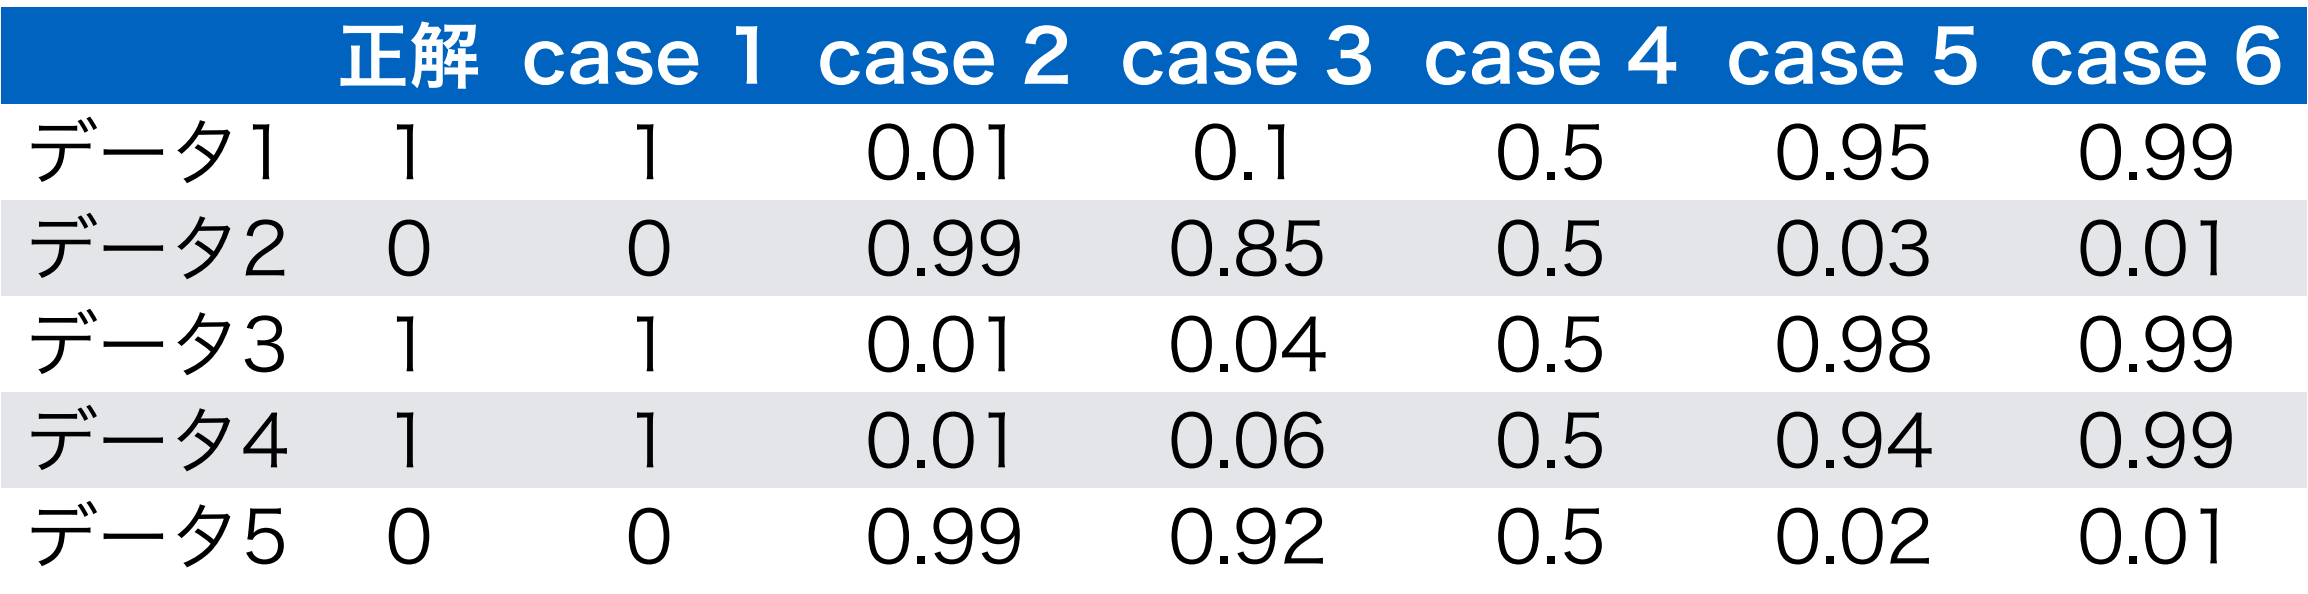
\includegraphics[scale=0.3]{./2023-06-23215207.png}
    \end{figure}

    \item クロスエントロピーと二乗平均誤差について、(2) で計算した値からわかる範囲で共通点と相違点について考察せよ。
    ただし、各ケースでの値を直接比較するのではなく、ケースの変化に対して値がどのように変化していくかについて考察すること。
    
\end{enumerate}

\subsection{制約条件}
この問題で求めるクロスエントロピーは、対数の底を $e$ としたものとすること。$0\log_{e}0$は数学においては本来計算不可能な量だが、
本問題においてもし出てきた場合には0としてよいものとする。


\section{問1} 
\subsection{問題文}
クロスエントロピーが計算可能であるためには、モデルの出力$\hat{y}$の値はある範囲内でなければならない。クロスエントロピーの式からその範囲がどのようになるか、説明せよ。
\subsection{解答}
結論から言えば、クロスエントロピーが計算可能であるためにはモデルの出力$\hat{y}$の値の範囲は、$0 < \hat{y} < 1$である必要がある。\par 
これは、クロスエントロピーの式とグラフを考えることで分かる。クロスエントロピーの式は以下のようになる。
\begin{equation}
    H(q, p) = -\sum_{x}q(x)\log_{e}p(x)\\
    \text{ここで、}q(x) = \text{正解ラベルの確率分布}p(x) = \text{予測値の確率分布} = \hat{y}
\end{equation}
分類問題において、クロスエントロピー誤差関数は、予測確率$p(x)$と正解ラベル$q(x)$の間の距離、不一致度を表す。
このとき、$q(x)$は、正解ラベルのみが1でそれ以外が0であるような確率分布であり、これはone-hotエンコーディングと呼ばれる。\par
ゆえに、ラベルの予測確率$p(x)$のみが誤差関数に影響を与えるので、分類問題ではクロスエントロピー誤差関数は、以下のような式になる。
\begin{equation}
    -\log_{e}p(x)
\end{equation}
このとき、クロスエントロピーのグラフは以下のようになる。
\begin{figure}[H]
    \centering
    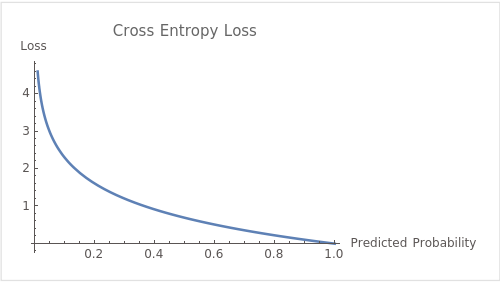
\includegraphics[scale=0.3]{./0ede6696-cbe7-4a39-b001-95edbb54e133.png}
\end{figure}
このグラフから、$p(x)$の値が0に近づくにつれて、その極限は無限大に発散していくことが分かる。従って、$p(x)$の値が0になることは許されない。
また、$p(x)$の値が1に近づくにつれて、その極限は0に収束していくことが分かる。クロスエントロピーの式から、$-\log_{e} 0 = \infty$であるため、
$p(x)$の値が1になることも許されない。\par
ゆえに、モデルの出力$\hat{y}$の値の範囲は、$0 < \hat{y} < 1$である必要がある。


\section{問2}
\subsection{問題文}
以下の表には、5つのデータからなる2値分類問題で、case 1~6 の6つの場合において、モデル出力がまとめられている。
それぞれのケースについて、5つのデータのクロスエントロピーの平均値を求めよ。\par 
また、各ケースの二乗平均誤差 (モデル出力と正解ラベルの差の二乗の平均値) も求めよ。
\begin{figure}[H]
    \centering
    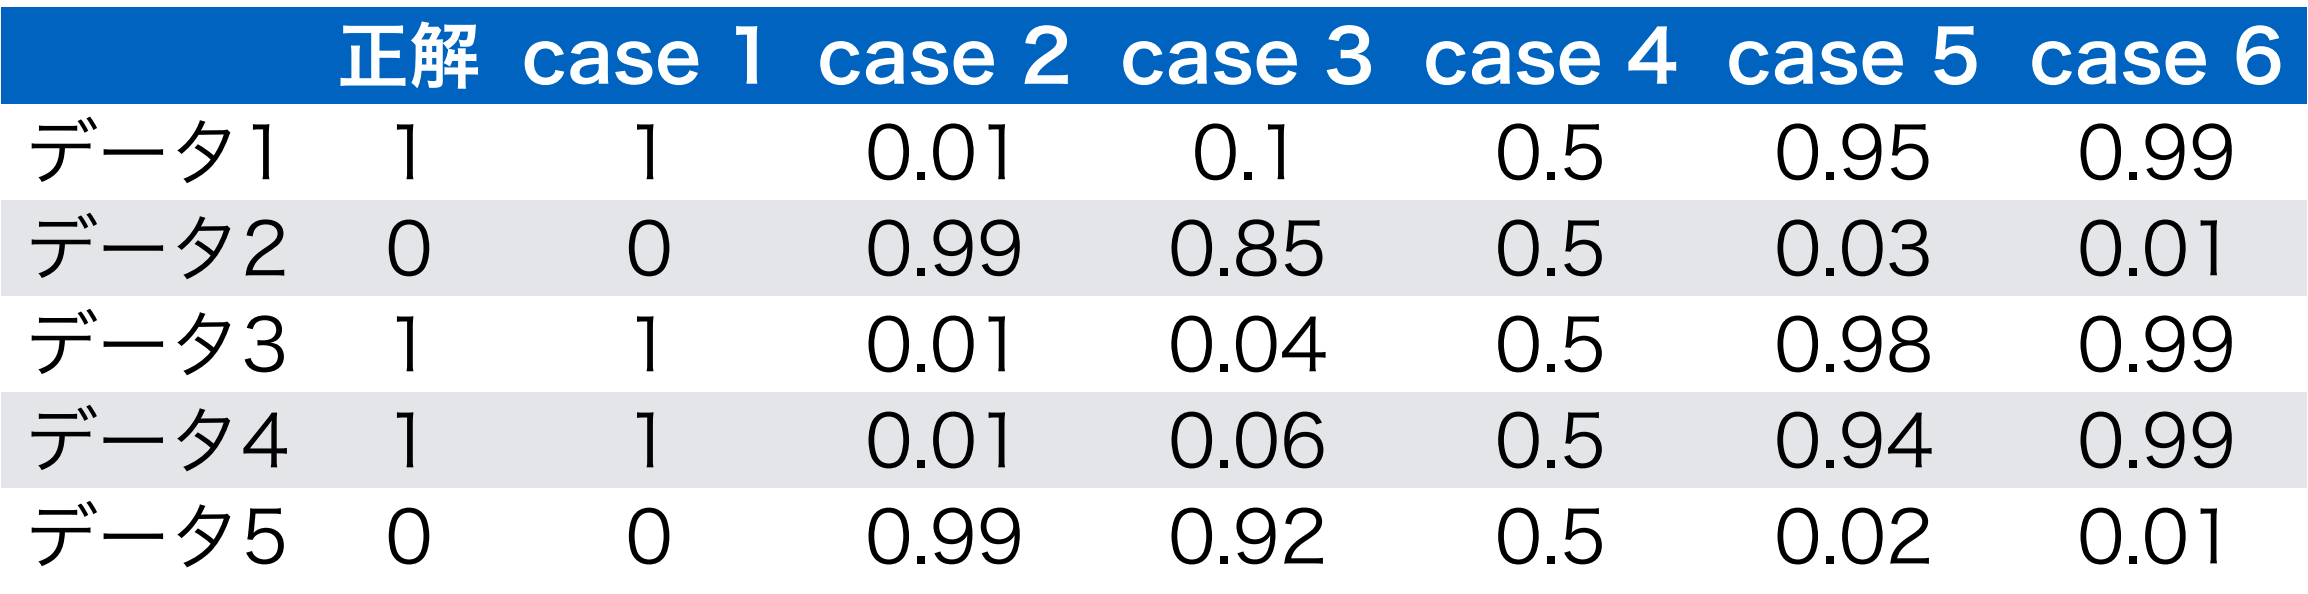
\includegraphics[scale=0.3]{./2023-06-23215207.png}
\end{figure}
\subsection{解答}
まず各データの、それぞれのケース毎にクロスエントロピーを計算した結果を以下に示す。
\data{データ1}
\begin{flalign*}
    
\end{flalign*}
\paragraph{case1}
\begin{flalign*}

\end{flalign*}
\section{問3}
\subsection{問題文}
クロスエントロピーと二乗平均誤差について、(2) で計算した値からわかる範囲で共通点と相違点について考察せよ。
ただし、各ケースでの値を直接比較するのではなく、ケースの変化に対して値がどのように変化していくかについて考察すること。
\subsection{解答}
\paragraph{データ1}
\begin{flalign*}
    
\end{flalign*}


  

\end{document}